\section{Sp\-Gpu\-Program.h File Reference}
\label{SpGpuProgram_8h}\index{SpGpuProgram.h@{SpGpuProgram.h}}
{\tt \#include \char`\"{}Sp\-Reference.h\char`\"{}}\par
{\tt \#include $<$memory$>$}\par
{\tt \#include \char`\"{}Sp\-Gpu\-Program.inc\char`\"{}}\par


Include dependency graph for Sp\-Gpu\-Program.h:\begin{figure}[H]
\begin{center}
\leavevmode
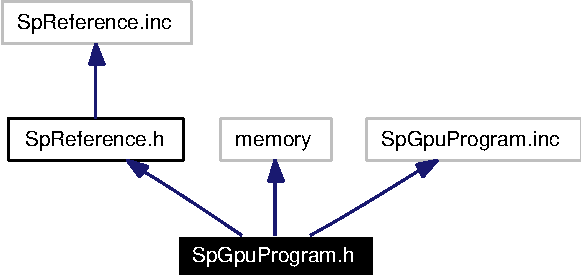
\includegraphics[width=157pt]{SpGpuProgram_8h__incl}
\end{center}
\end{figure}


This graph shows which files directly or indirectly include this file:\begin{figure}[H]
\begin{center}
\leavevmode
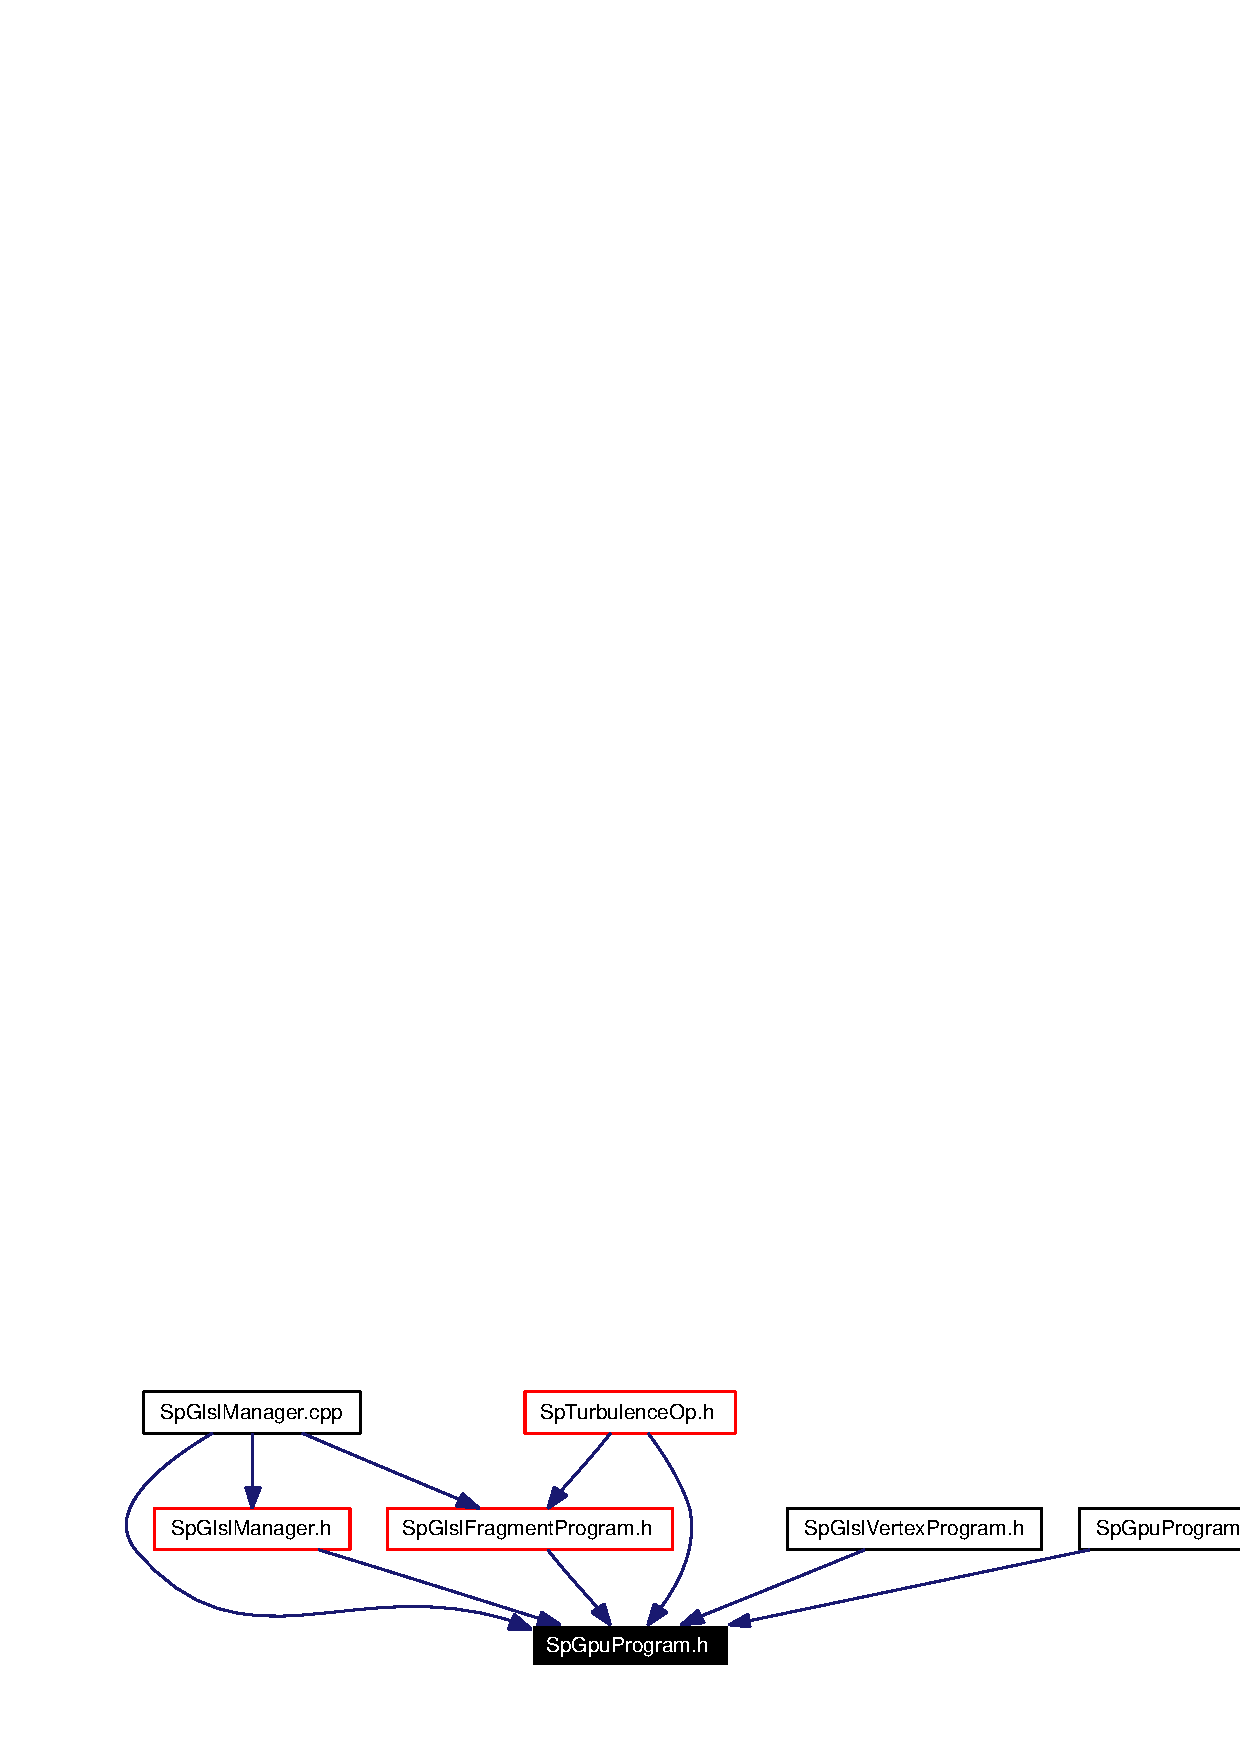
\includegraphics[width=312pt]{SpGpuProgram_8h__dep__incl}
\end{center}
\end{figure}
\subsection*{Namespaces}
\begin{CompactItemize}
\item 
namespace {\bf Spark}
\end{CompactItemize}
\subsection*{Classes}
\begin{CompactItemize}
\item 
class {\bf Spark::Sp\-Gpu\-Program}
\begin{CompactList}\small\item\em Abstract base class for a GPU program. \item\end{CompactList}\end{CompactItemize}
\subsection*{Typedefs}
\begin{CompactItemize}
\item 
typedef Sp\-Reference$<$ {\bf Sp\-Gpu\-Program} $>$ {\bf Sp\-Gpu\-Program\-Ptr}
\end{CompactItemize}


\subsection{Typedef Documentation}
\index{SpGpuProgram.h@{Sp\-Gpu\-Program.h}!SpGpuProgramPtr@{SpGpuProgramPtr}}
\index{SpGpuProgramPtr@{SpGpuProgramPtr}!SpGpuProgram.h@{Sp\-Gpu\-Program.h}}
\subsubsection{\setlength{\rightskip}{0pt plus 5cm}typedef Sp\-Reference$<$ {\bf Sp\-Gpu\-Program} $>$ {\bf Spark::Sp\-Gpu\-Program\-Ptr}}\label{namespaceSpark_a0}


Definition at line 152 of file Sp\-Gpu\-Program.h.

Referenced by Spark::Sp\-Gpu\-Program::get\-Source().